\section{Time Difference Of Arrival}
\label{sec:02_tdoa}

The direction of a signal source $\gamma'$ can be determined by the time
delay of the received signal.
Calculations for the direction of the sound source can be done with a
geometrical approach like in \cite{Valin_Michaud}.
\Cref{fig:02_tdoa} illustrates how a the delay $D$ introduced by the direction angle
of the sound source relative to a vector between channels 0 and 1.
Here, the signal arrives first at channel 0. Ideally, the same signal values
are measured at channel 1 with delay $D$.
If the delay is zero, the signal is perpendicular to the channels vector.
It's value can be $D_{max}$ maximally which in that case delivers the
result of the source direction vector being aligned to the channels vector.
It is assumed that the distance from the sensors to the sound source is
significantly large so that the signal waves proceed parallel which is a necessary
criterion for the approach to be valid.
\begin{figure}[ht]
	\centering
		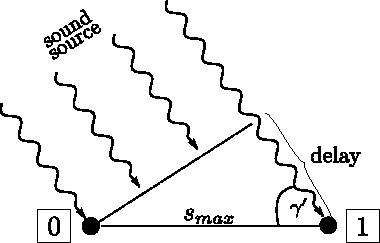
\includegraphics[width=0.4\columnwidth]{figures/tdoa_waves}
	\caption{Illustration of TDOA principle.}
    \label{fig:02_tdoa}
\end{figure}
% -------------------------------------------------------------

Specifying the speed of sound $c_s$ being 343\si{m/s} in air, the angle
$\gamma'$ can be defined as
\bsub \bal
    \gamma' &= cos^{-1}(\frac{|D|}{D_{max}})
    \label{eq:02_tdoaAngle}\\
    \intertext{with}
    D_{max} &= \frac{f_s * d_{01}}{c_s}
\eal \esub
where $f_s$ is the sampling rate and $d_{01}$ is the distance between both channel.
Not to forget is the ambiguity of the result by observing two channel only.
Having a look at \cref{fig:02_tdoa} once more and assuming that the sound source
is positioned in front, the same delay can be the result of a sound source from behind.

% -------------------------------------------------------------

With the definition of a whistle signal as stated in \cref{eq:02_whistleSignal},
the microphone sensors $channel_0$ and $channel_1$ will output
\bsub
\label{eq:02_signalTimeDomain}
\bal
    x_0(t) &= s(t) + n_0(t)\\
    x_1(t) &= \alpha s(t - D) + n_1(t).
\eal \esub
Again, $D$ is the delay of $x_1$ relative to $x_0$ for what is looked for.
As introduced in \cref{chap:01_introduction}, different methods to detect this delay
were implemented and evaluated in this work.
In the following sections, the theoretical background of these will be
explained in detail.